\documentclass[xcolor=dvipsnames,handout]{beamer}

\usepackage[utf8x]{inputenc}
\usepackage{default}
\usetheme[width=50pt]{ULatina}   % Bergen, Darmstadt
\usecolortheme[named=Green]{structure}
\usepackage{graphicx}
\usepackage{pgfpages}
\usepackage{tikz}
\usepackage[spanish]{babel}

\newcommand{\uC}{\ensuremath{\mu\textrm{C}}\ }
\newcommand{\pageframe}[1]{\frame{\begin{center}{ \Huge #1 }\end{center}}}
%\setbeameroption{show notes on second screen}

\title[PIC16]{Microcontroladores PIC16}
\subtitle[ASM]{Fundamentos de ASM}
\author{Prof. Jorge Rivera~Guti\'errez}
\institute{Universidad Latina de Costa Rica\\ Ingenier\'\i a en Electr\'onica}
\logo{
\includegraphics[height=45pt]{world.png}}
\date{III Cuatrimestre 2013}


\begin{document}

\begin{frame}
 \maketitle
\end{frame}

\begin{frame}
 \tableofcontents[pausesections]
\end{frame}


\section{Arquitectura de PIC16}
\pageframe{Arquitectura de la familia PIC16}
\begin{frame}[t]
  \frametitle{Diagrama de bloques}
      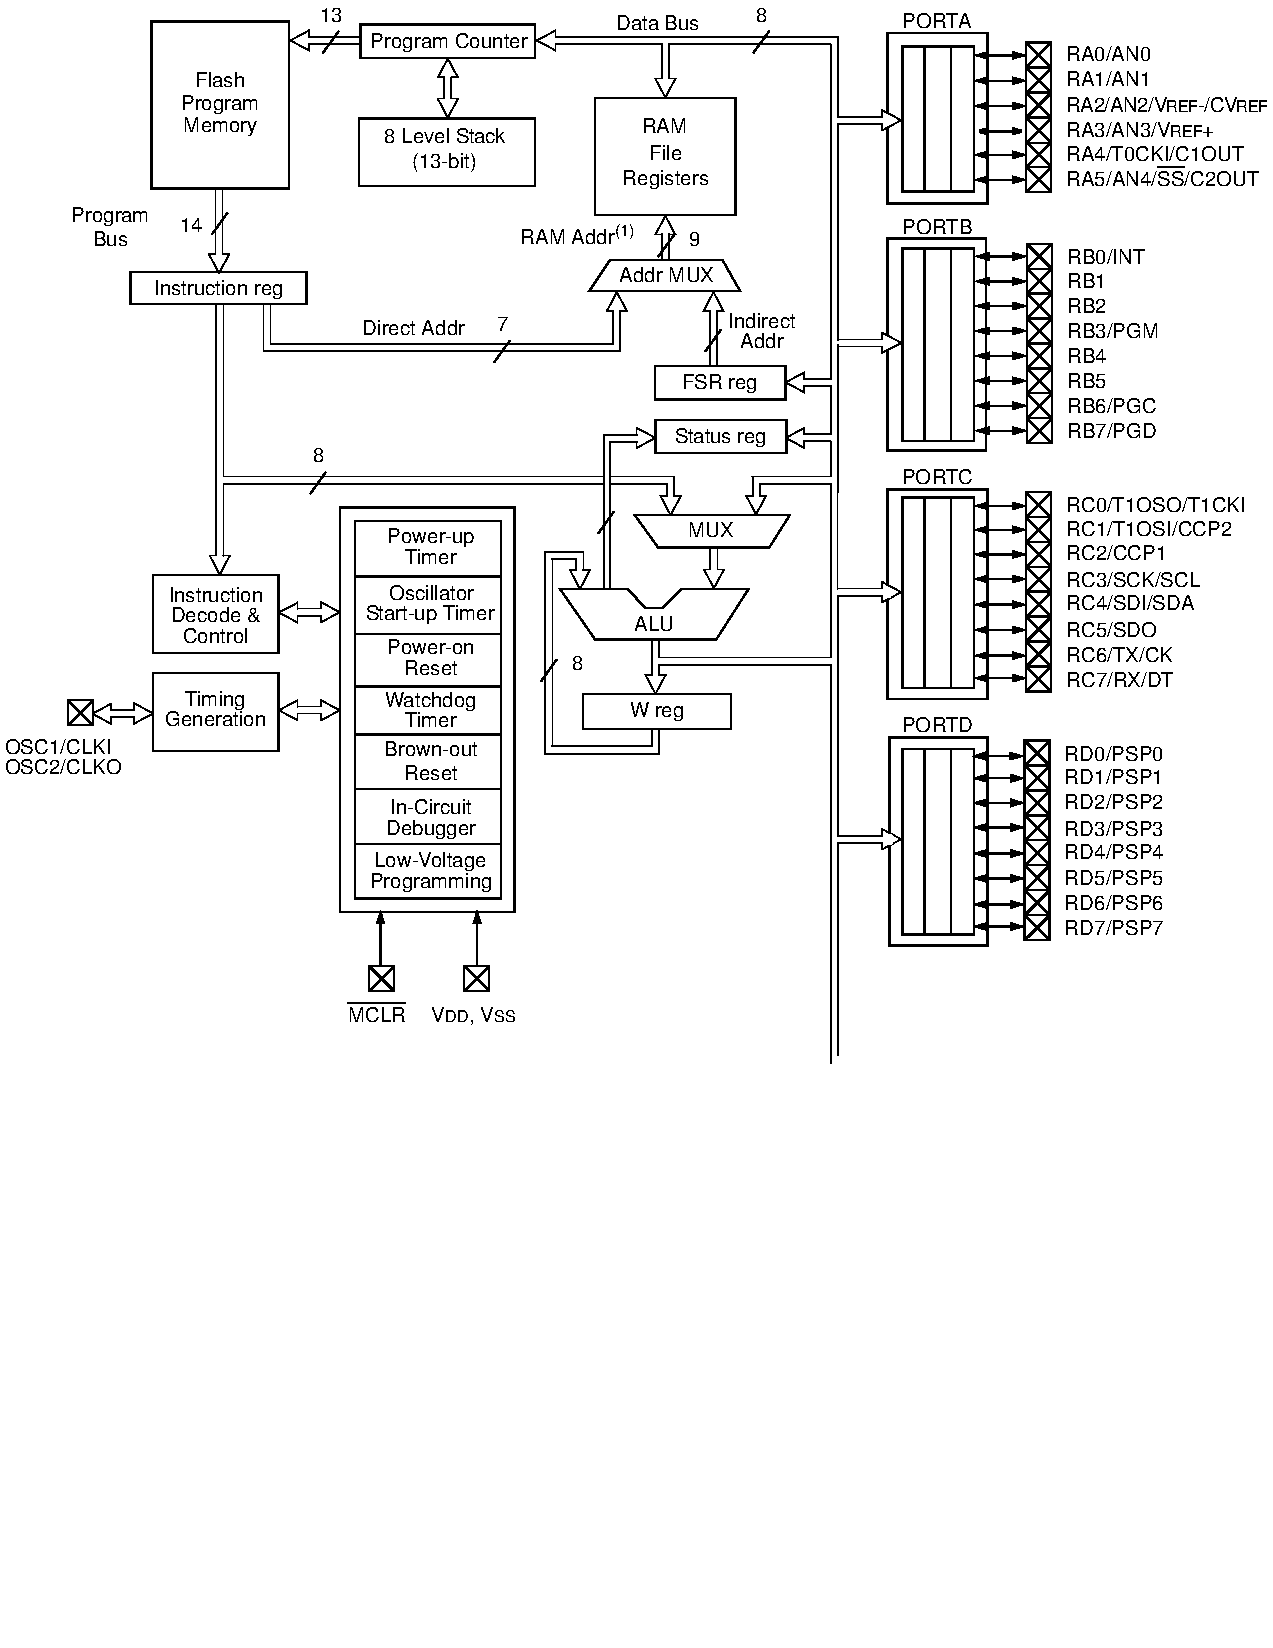
\includegraphics[width=.9\textwidth]{BlockDiagram}
\end{frame}

\subsection{Mapa de Registros}
\pageframe{Mapa de Registros}
\begin{frame}[t]
  \frametitle{Mapa de Registros}
  \begin{center}
    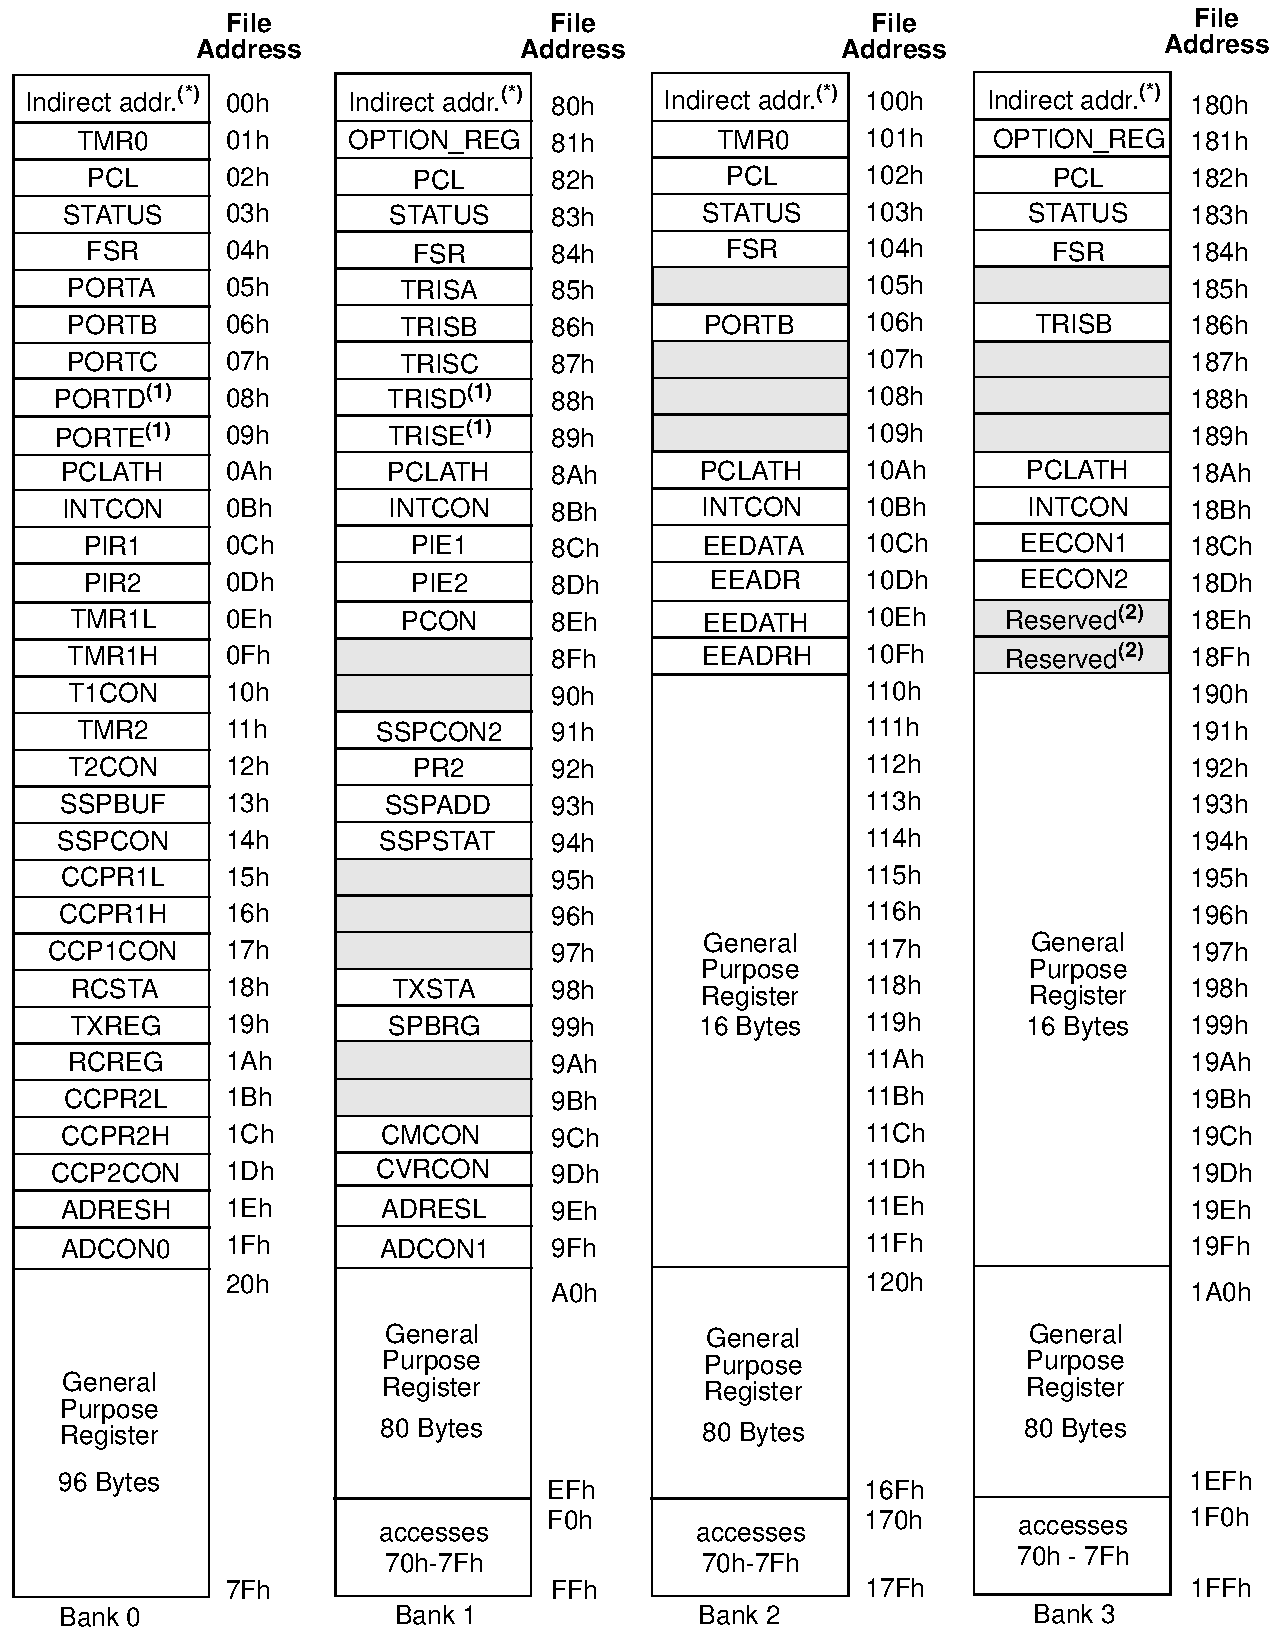
\includegraphics[width=.55\textwidth]{DataMemMap}
  \end{center}

\end{frame}

\subsection{Mapa de memoria de programa}
\pageframe{Mapa de memoria de programa}
\begin{frame}[t]
  \frametitle{Mapa de memoria de programa}
  \begin{center}
    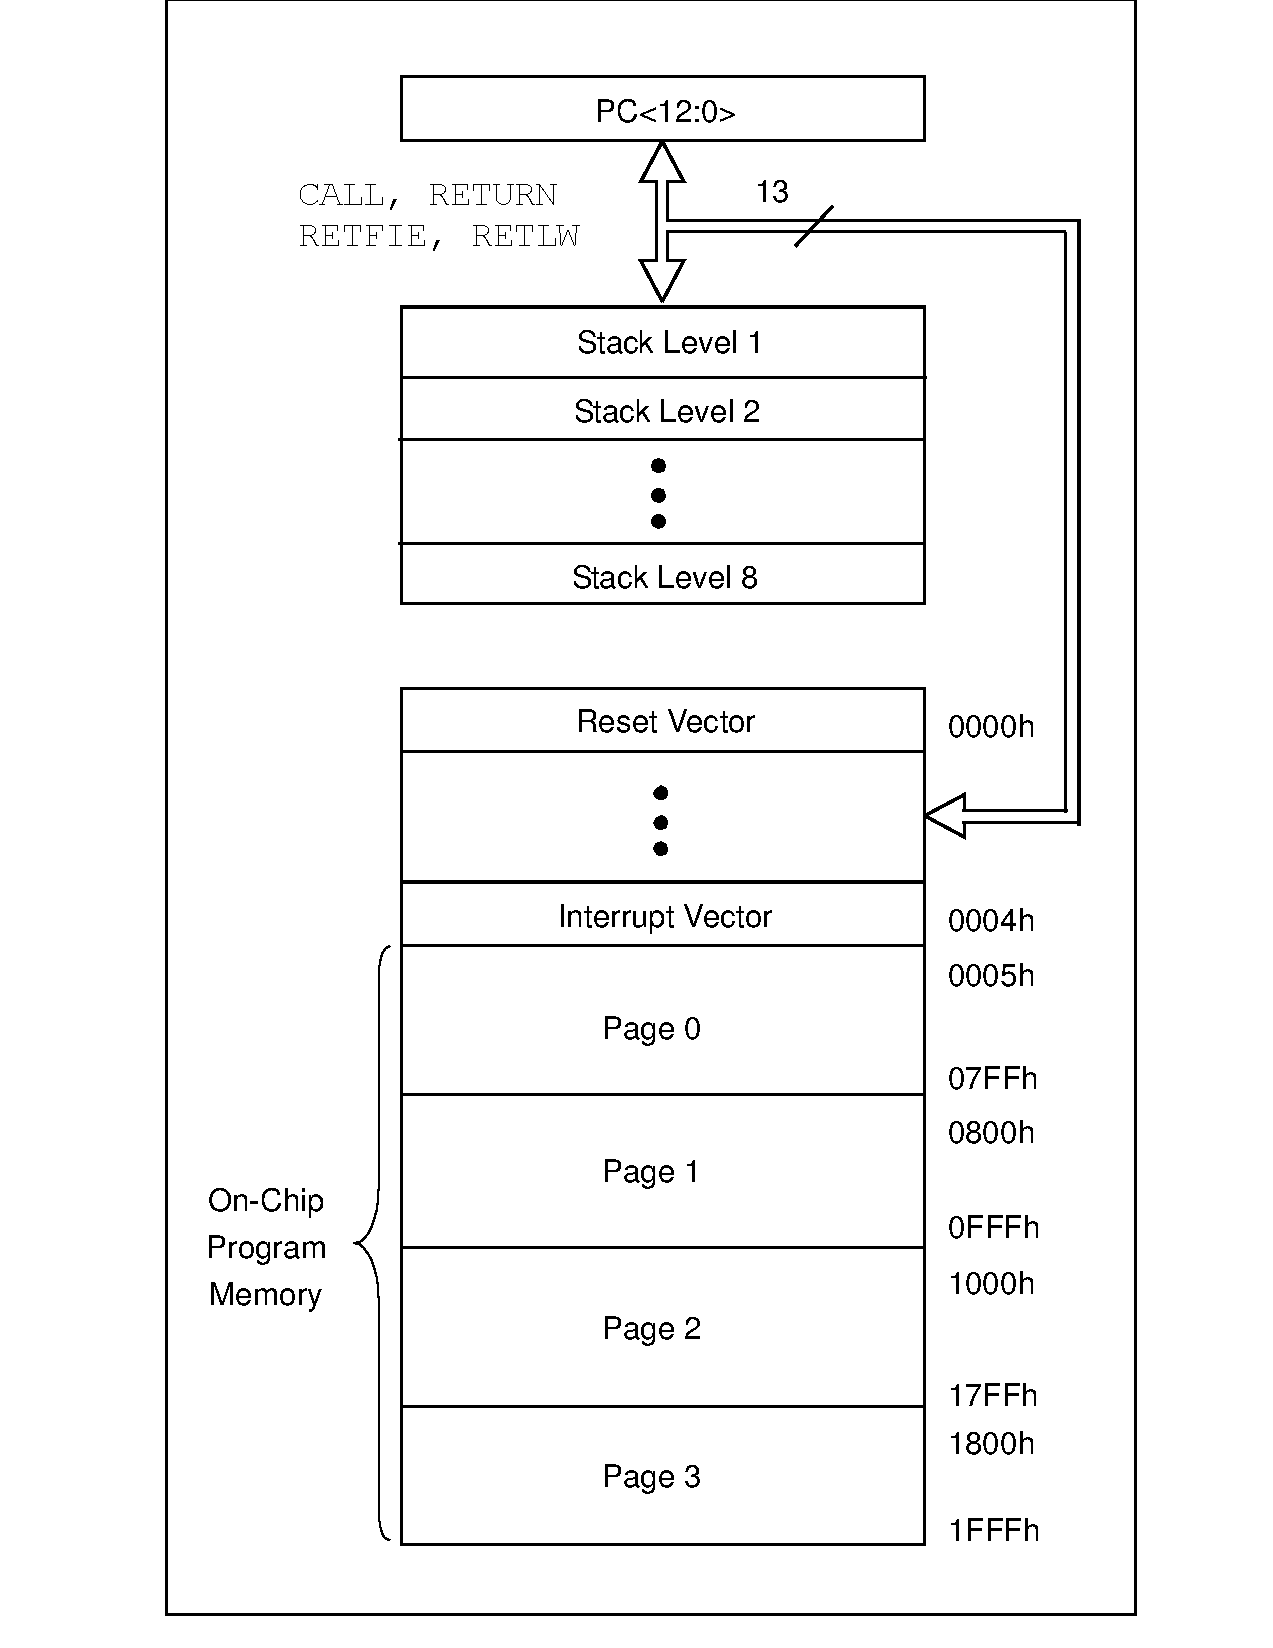
\includegraphics[width=.55\textwidth]{ProgMemMap}
  \end{center}
\end{frame}

\subsection{Registro de Configuraci\'on}
\pageframe{Registro de configuraci\'on}
\begin{frame}[t]
  \frametitle{Registro de Configuración}
  \begin{center}
    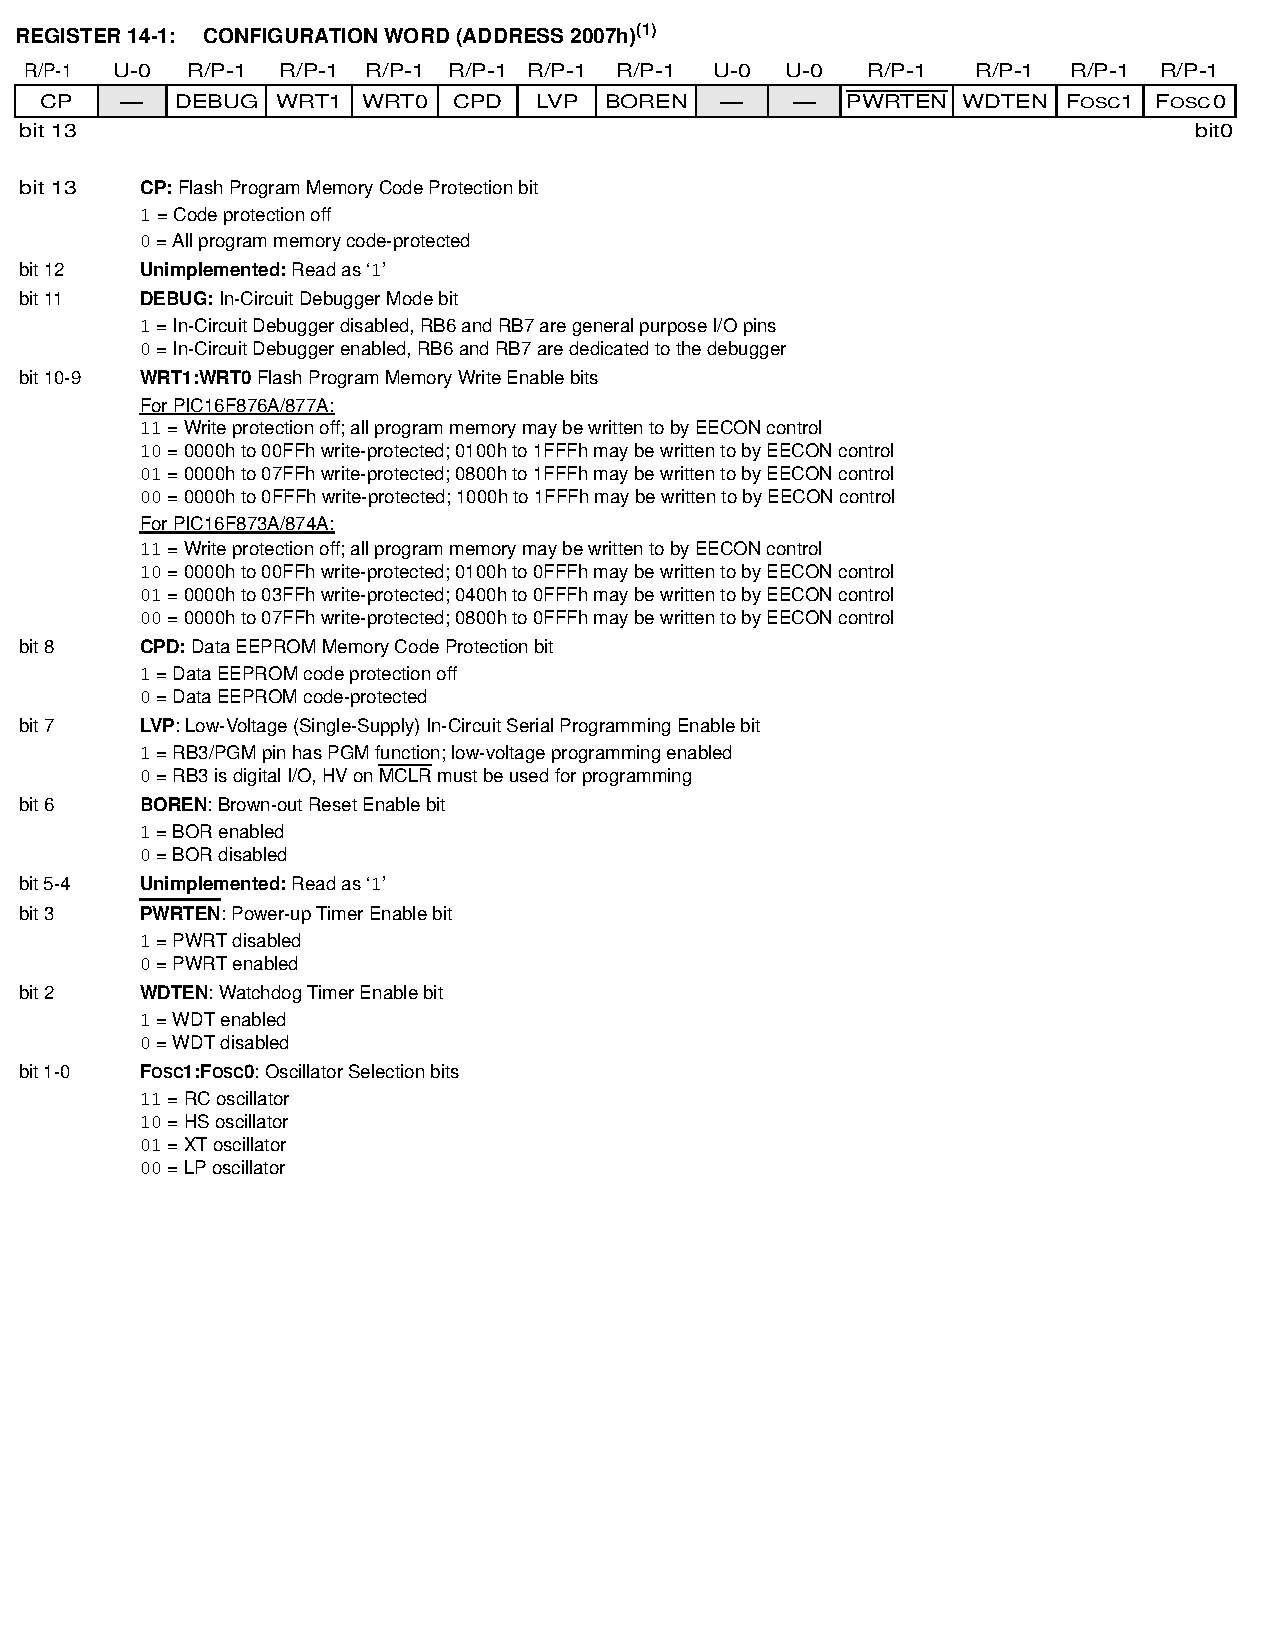
\includegraphics[width=.80\textwidth]{ConfigWord}
  \end{center}

\end{frame}

\section{Ensamblador}

\pageframe{Instrucciones con W y literal} % son 8
\begin{frame}{MOVLW, CLRW}
  \begin{block}{MOVLW -- Move Literal to W}
      \begin{itemize}
	\item\textbf{Syntax} MOVLW $k$
	\item\textbf{Operands} $0\leq k\leq 255$
	\item\textbf{Operation} $k\rightarrow (W)$
	\item\textbf{Description} El contenido del literal de ocho bits $k$ se almacena en W.
      \end{itemize}      

  \end{block}
\end{frame}

\begin{frame}{ADDLW, ANDLW, IORLW, SUBLW, XORLW}
  \begin{block}{ADDLW -- Add Literal and W}
      \begin{itemize}
	\item\textbf{Syntax} ADDLW $k$
	\item\textbf{Operands} $0\leq k\leq 255$
	\item\textbf{Operation} $(W)+k\rightarrow (W)$
	\item\textbf{Status Affected} C, DC, Z
	\item\textbf{Description} El contenido de W se suma al literal de ocho bits $k$ y el resultado se almacena en W.
      \end{itemize}      
  \end{block}
\end{frame}

\begin{frame}{RETLW}
  \begin{block}{RETLW -- Return with literal}

      \begin{itemize}
	\item\textbf{Syntax} RETLW $k$
	\item\textbf{Operands} $0\leq k\leq 255$
	\item\textbf{Operation} $k\rightarrow (W)$, TOS$\rightarrow$ PC
	\item\textbf{Description} El contenido del literal de ocho bits $k$ se almacena en W y se retorna a la ubicación almacenada en TOS.
      \end{itemize} 
  \end{block}
\end{frame}



\pageframe{Instrucciones con W y un registro f} % son 9
\begin{frame}{MOVF, MOVWF, CLRF}
  \begin{block}{MOVWF -- Move W to f}
      \begin{itemize}
	\item\textbf{Syntax} MOVWF $f$
	\item\textbf{Operands} $f$
	\item\textbf{Description} El contenido de W se almacena en el registro $f$.
      \end{itemize}      

  \end{block}
\end{frame}

\begin{frame}{ADDWF, ANDWF, IORWF, SUBWF, XORWF}
   \begin{block}{ADDWF -- Add W and f}
      \begin{itemize}
	\item\textbf{Syntax} ADDWF $f, d$
	\item\textbf{Operands} $0\leq f\leq 255$, $d\in [0,1]$
	\item\textbf{Operation} $(W)+(f)\rightarrow (\textrm{dest})$
	\item\textbf{Status Affected} C, DC, Z
	\item\textbf{Description} El contenido de W se suma al contenido del registro $f$. Si $d$ es 0, se almacena en W. Si $d$ es 1, se almacena en el registro $f$.
      \end{itemize}      
  \end{block}

\end{frame}


\pageframe{Instrucciones sobre un registro f} % son 9

\begin{frame}{DECF, COMF, INCF, RLF, RRF, SWAPF}
   \begin{block}{DECF -- Decrement f}
      \begin{itemize}
	\item\textbf{Syntax} DECF $f, d$
	\item\textbf{Operands} $0\leq f\leq 255$, $d\in [0,1]$
	\item\textbf{Operation} $(f)-1\rightarrow (\textrm{dest})$
	\item\textbf{Status Affected} C, DC, Z
	\item\textbf{Description} El contenido de $f$ se decrementa en 1. Si $d$ es 0, se almacena en W. Si $d$ es 1, se almacena en el registro $f$.
      \end{itemize}      
  \end{block}

\end{frame}

\begin{frame}{DECFSZ, INCFSZ}
   \begin{block}{DECFSZ -- Decrement f, skip if 0}
      \begin{itemize}
	\item\textbf{Syntax} DECFSZ $f, d$
	\item\textbf{Operands} $0\leq f\leq 255$, $d\in [0,1]$
	\item\textbf{Operation} $(f)-1\rightarrow (\textrm{dest})$; skip if result = 0
	\item\textbf{Description} El contenido de $f$ se decrementa en 1. Si $d$ es 0, se almacena en W. Si $d$ es 1, se almacena en el registro $f$. 

	Si el resultado es 1, se ejecuta la siguiente instrucción. Si es 0 se ejecuta un NOP y se duran 2 $T_{CY}$ en la ejecución.
      \end{itemize}      
  \end{block}

\end{frame}



\pageframe{Instrucciones orientadas a bits}  % son 4

\begin{frame}{BCF, BSF}
   \begin{block}{BCF -- Bit clear f}
      \begin{itemize}
	\item\textbf{Syntax} BCF $f, b$
	\item\textbf{Operands} $0\leq f\leq 255$, $0\leq b\leq 7$
	\item\textbf{Operation} $0\rightarrow (f<b>)$
	\item\textbf{Description} El bit $b$ del registro $f$ se pone en cero.
      \end{itemize}      
  \end{block}
\end{frame}

\begin{frame}{BTFSC, BTFSS}
   \begin{block}{BTFSC -- Bit test f, Skip if Clear}
      \begin{itemize}
	\item\textbf{Syntax} BTFSC $f, b$
	\item\textbf{Operands} $0\leq f\leq 255$, $0\leq b\leq 7$
	\item\textbf{Operation} skip if $(f<b>)=1$
	\item\textbf{Description} Si el bit $b$ del registro $f$ es 0, se ejecuta la siguiente instrucción.

	Si el bit $b$ es 1, la siguiente instrucción se descarta y se ejecuta un NOP. La duración en este caso es 2$T_{CY}$.
      \end{itemize}      
  \end{block}

\end{frame}



\pageframe{Instrucciones de control de flujo}  % son 4

\begin{frame}{CALL, GOTO, RETURN, RETFIE}
    \begin{block}{GOTO -- Saltar a una posición de memoria}
      \begin{itemize}
	\item\textbf{Syntax} GOTO $k$
	\item\textbf{Operands} $0\leq k\leq 2047$
	\item\textbf{Operation} $k\rightarrow PC<10:0>$, $(PCLATH<4:3>)\rightarrow PC<12:11>$
	\item\textbf{Description} Saltar a posición de memoria. La dirección de 11 bits $k$ se almacena en $PC<10:0>$. Los bits más altos de PC se cargan de $PCLATH<4:3>$.
      \end{itemize}      
  \end{block}
\end{frame}

\pageframe{Instrucciones sin operandos} % son 3

\begin{frame}{NOP, SLEEP, CLRWDT}
\only<1>{
     \begin{block}{NOP -- No operation}
      \begin{itemize}
	\item\textbf{Syntax} NOP
	\item\textbf{Operation} Ninguna
	\item\textbf{Description} No realiza ninguna operación.
      \end{itemize}      
  \end{block}
}
\end{frame}
\begin{frame}{NOP, SLEEP, CLRWDT}
\only<1>{
     \begin{block}{SLEEP -- Entrar en modo sleep }
      \begin{itemize}
	\item\textbf{Syntax} SLEEP
	\item\textbf{Operation} $00h\rightarrow WDT$,

	$0\rightarrow WDT\textrm{ prescaler}$, 

	$1\rightarrow \overline{TO}$,

	$0\rightarrow \overline{PD}$,


	\item\textbf{Description} El bit de Power Down se pone 0. Timeout en 1. El WDT se limpia. El procesador se duerme con el oscilador se detiene.
      \end{itemize}      
  \end{block}
}

\end{frame}

\section[Retos]{Retos de programaci\'on}

\pageframe{Retos de programación}

\subsection[L\'ogica]{Simulación de compuerta l\'ogica}

\begin{frame}{Compuerta Lógica AND}%$a \& b$}
\begin{block}{Compuerta Lógica AND}
\begin{center}
¿Cómo simular una compuerta lógica tipo AND de dos entradas?
\end{center} 
\end{block}
\end{frame}



\subsection[Trigonometr\'\i a]{C\'alculo de operaciones trigonom\'etricas}

\begin{frame}{Seno de un ángulo}%$\sin \thetha$}
\begin{block}{Seno de un ángulo}

\begin{center}
¿Cómo calcular el seno de un ángulo entre 0 y 90 grados?
\end{center} 
\end{block}
\end{frame}

\subsection[Switch]{Implementaci\'on de ``switch''}

\begin{frame}{Implementaci\'on de ``switch''}
\begin{block}{Switch, case}

\begin{center}
¿Cómo construir un switch?
\end{center} 
\end{block}
\end{frame}

\end{document}
